\begin{sidewaysfigure*}
\thisfloatpagestyle{mylandscape}%
\rotatesidewayslabel%
\centering
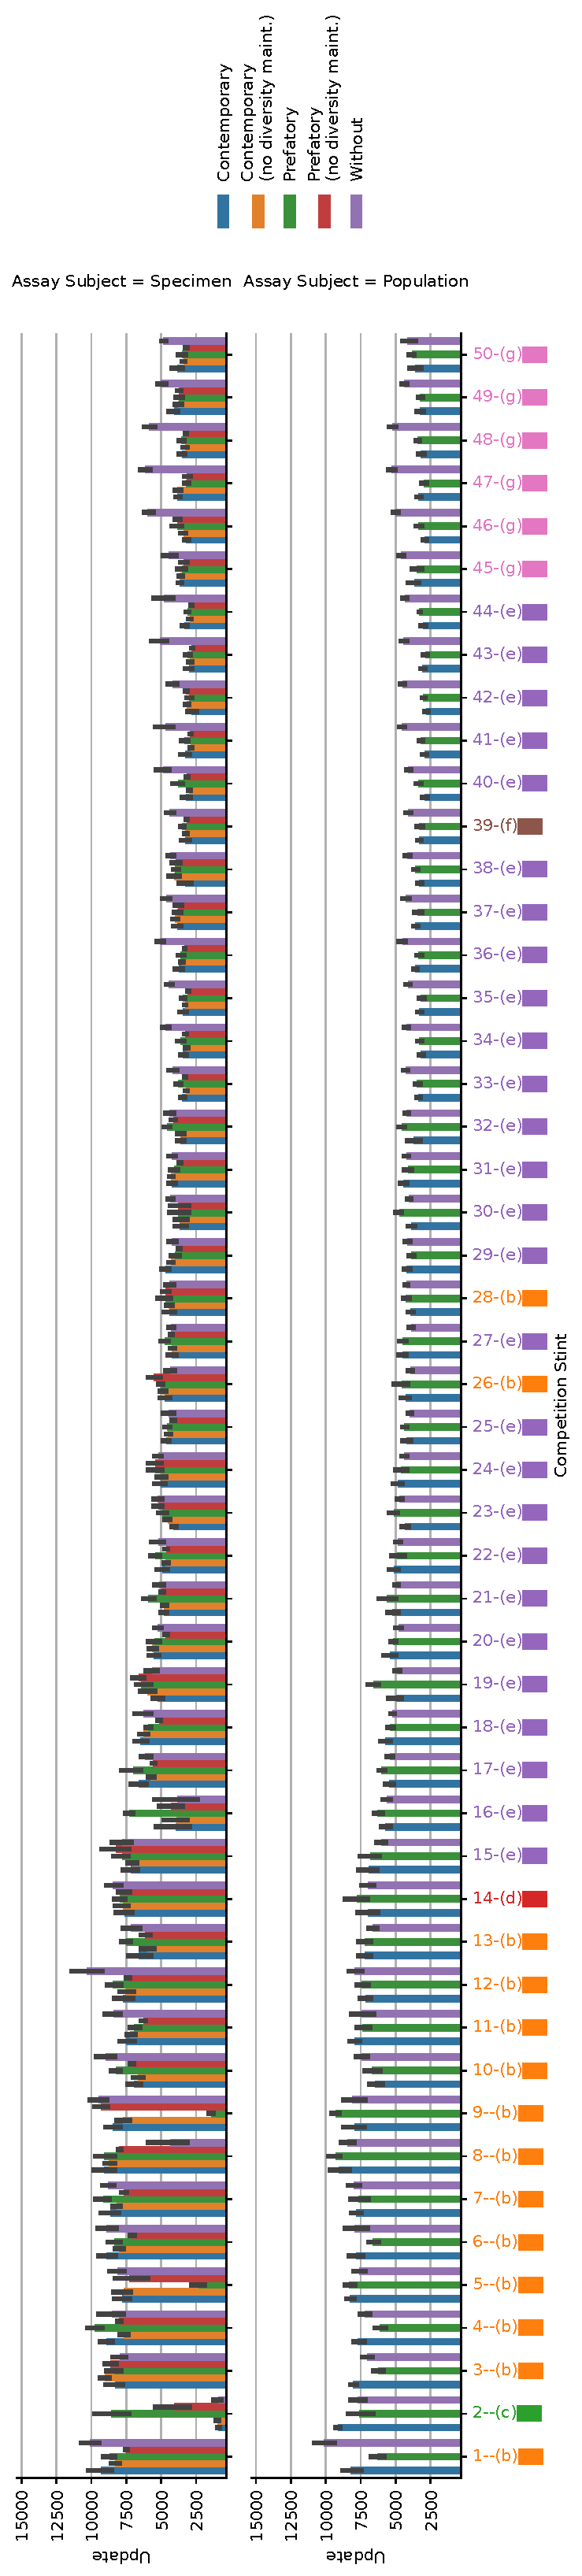
\includegraphics[width=\linewidth]{{submodule/dishtiny/binder/bucket=prq49/a=adaptation_assays+endeavor=16/teeplots/hue=biotic-background+stint=1-50+viz=facet-barplot+x=competition-stint+y=update+ext=}}
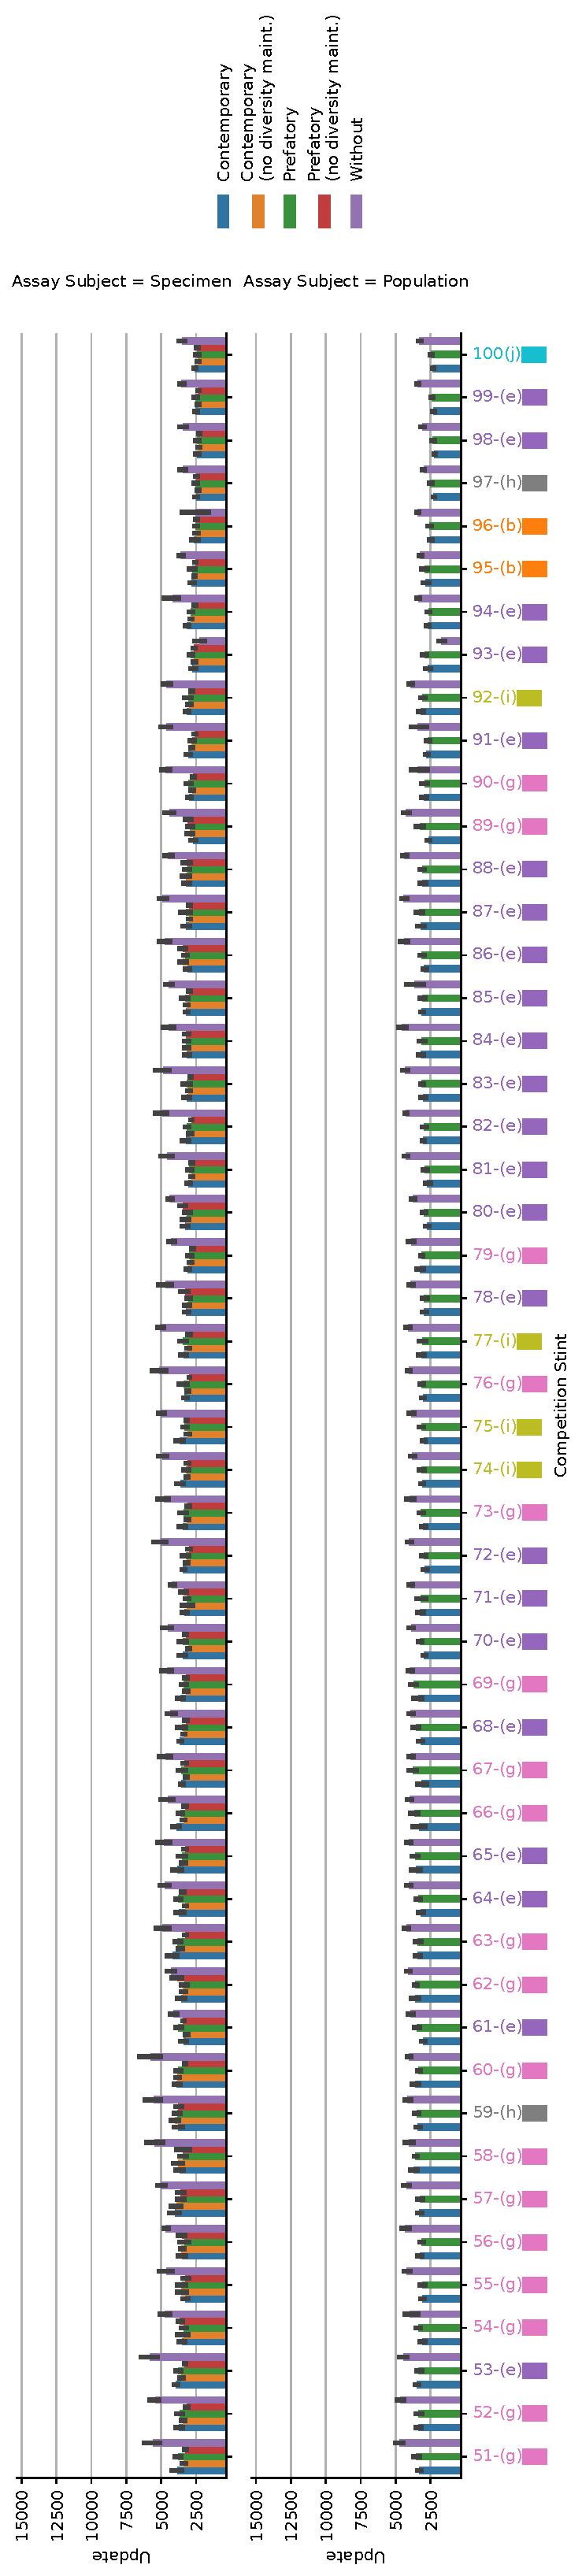
\includegraphics[width=\linewidth]{{submodule/dishtiny/binder/bucket=prq49/a=adaptation_assays+endeavor=16/teeplots/hue=biotic-background+stint=51-100+viz=facet-barplot+x=competition-stint+y=update+ext=}}

\caption{
\textbf{Number updates elapsed during fixed-duration adaptation assay competitions.}
\footnotesize
For sampled representative specimen (upper panels) population-level adaptation (lower panels).
Error bars are bootstrapped 95\% confidence intervals.
Figure is split into two rows due to layout considerations.
See Figure \ref{fig:adaptation_assay_cartoon} for explanation of competition biotic backgrounds.
}
\label{fig:num_updates_elapsed_barplot}
\end{sidewaysfigure*}
